\documentclass[10pt]{beamer}
\usepackage[utf8]{inputenc}
\usepackage{polski}
\usepackage{verbatim}
\usepackage{subfigure}
%\usepackage{amsfonts}
%\usepackage{amssymb}
%\usepackage{alltt}
\usepackage{color, graphicx}
\usepackage{array}
\usepackage{epstopdf}
%\usepackage{animate}
\pdfpageattr {/Group << /S /Transparency /I true /CS /DeviceRGB>>}

\usecolortheme[RGB={0,200,0}]{structure}
\usetheme{Frankfurt}

\author{Mateusz Najsztub}
\title{Odzyskiwanie parametrów kinetycznych rozplatania kinazy tytyny 1TKI z symulacji dynamiki molekularnej}
%\institute{Laboratory for Dynamics of Physicochemical Processes}
\begin{document}

\begin{frame}[plain]

\titlepage
\end{frame}


\section{Symulacje}

\subsection{Procedura}

\begin{frame}
\frametitle{Schemat postępowania}
	\begin{figure}
		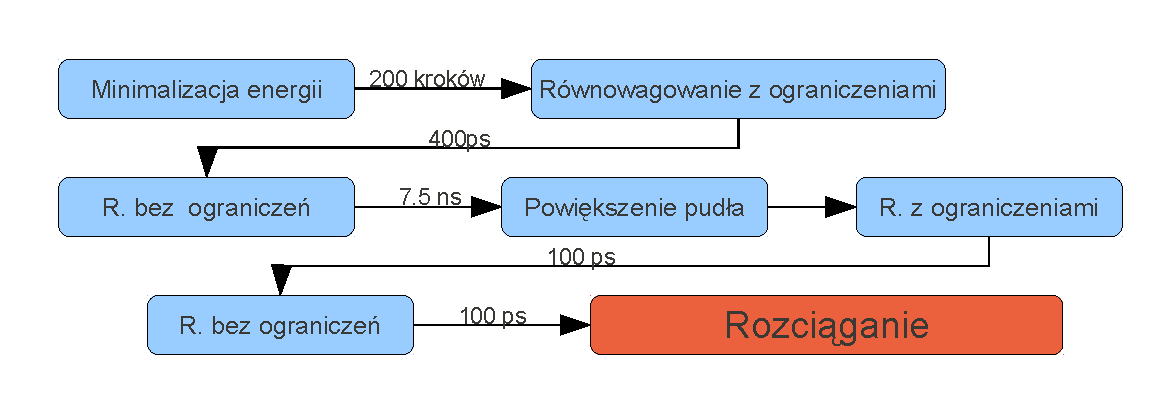
\includegraphics[height = 0.35\textwidth]{rys/schemat.pdf} 
		\caption{Schemat postępowania}
	\end{figure}
\end{frame}

\begin{frame}
\frametitle{Układ}
\begin{center}
\begin{figure}[h]
\begin{centering}
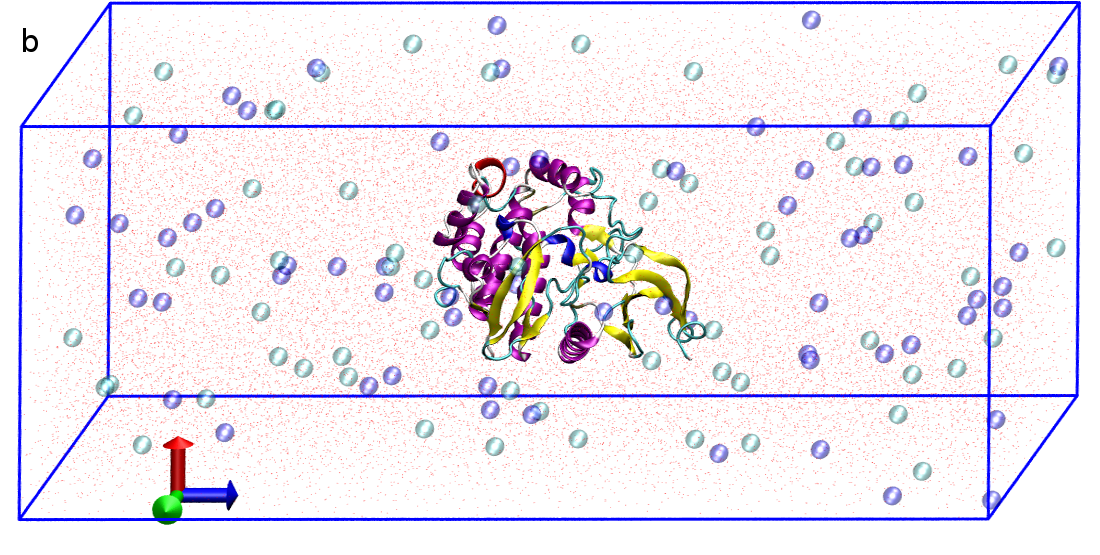
\includegraphics[width=100mm]{./rys/plot.png}
\caption{Wizualizacja układu.}
\end{centering}
\end{figure}
\end{center}
\end{frame}

\subsection{Parametry}



\begin{frame}
\frametitle{Parametry}
\begin{block}{Parametry}
\begin{enumerate}
\item Pudełko: 8.8 x 7.8 x 7.6 nm, później 7.8 x 8.4 x 18.6 nm
\item Termostat (300K) i barostat (1 bar)
\item Pole siłowe: GROMOS
\item Woda: SPC
\item Rozpuszczalnik: siła jonowa 100 mM
\item Protonowanie: WHATIF
\end{enumerate}

\end{block}
\end{frame}

\begin{frame}
\frametitle{Różnice}
\begin{block}{Różnice}
\begin{enumerate}
\item Termostat Berendsena; V-Rescale
\item Barostat dla x, y, z; tylko dla x i y
\item Kod rozciągania pisany ręcznie; kod direction\_periodic
\item Wersja Gromacsa 3.3; wersja 4.5
\end{enumerate}

\end{block}
\end{frame}

\begin{frame}
\frametitle{Wykres RMSD, p, V i T od t}
	\begin{figure}
		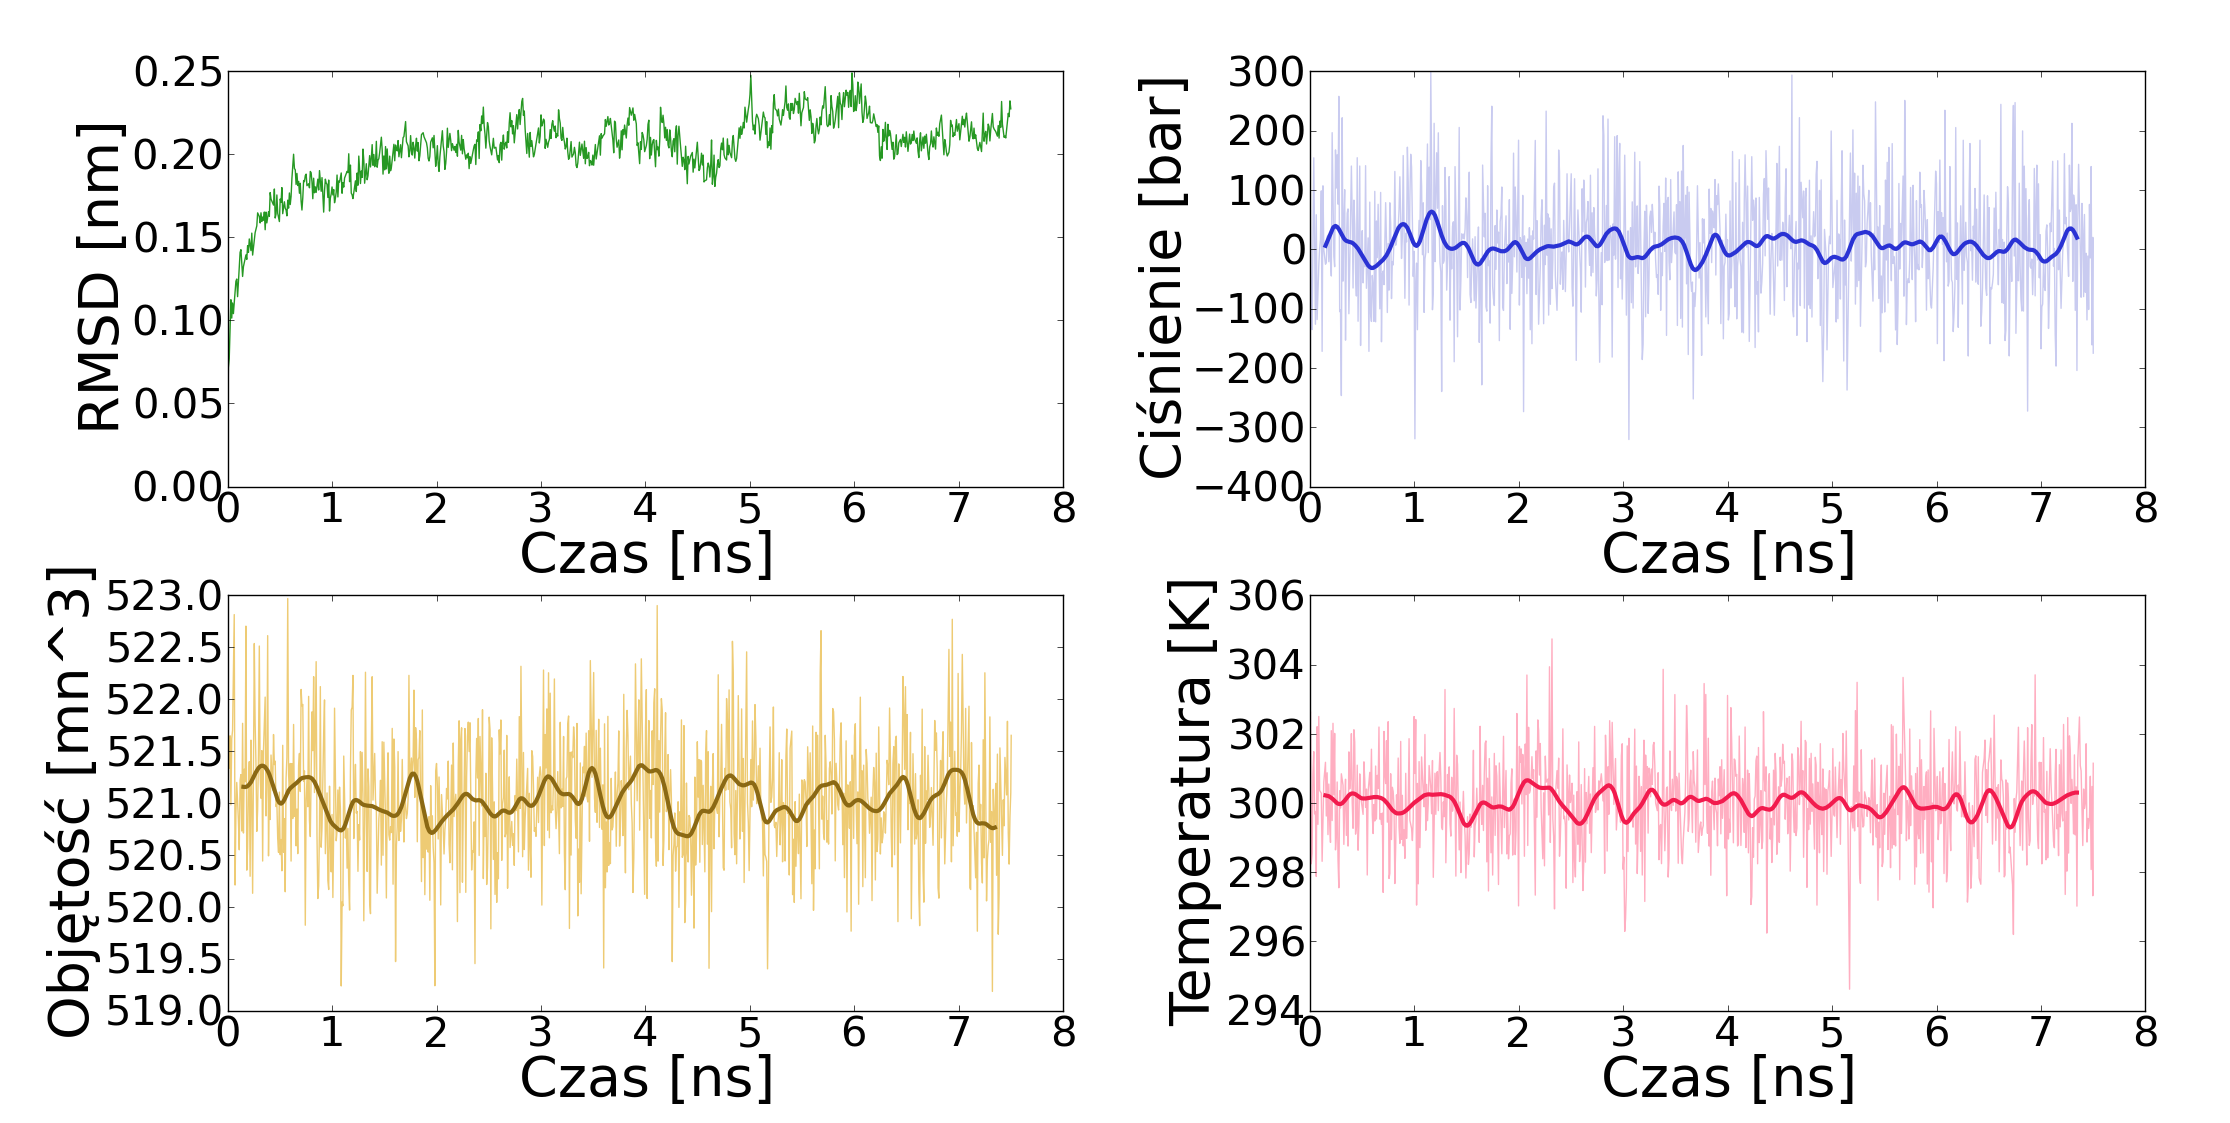
\includegraphics[height = 0.5\linewidth]{rys/rmsd.png} 
		\caption{Wykres RMSD, p, V i T od t}
	\end{figure}
\end{frame}



\begin{frame}
\frametitle{Wygładzanie}
\begin{center}
\begin{figure}[h]
\begin{centering}
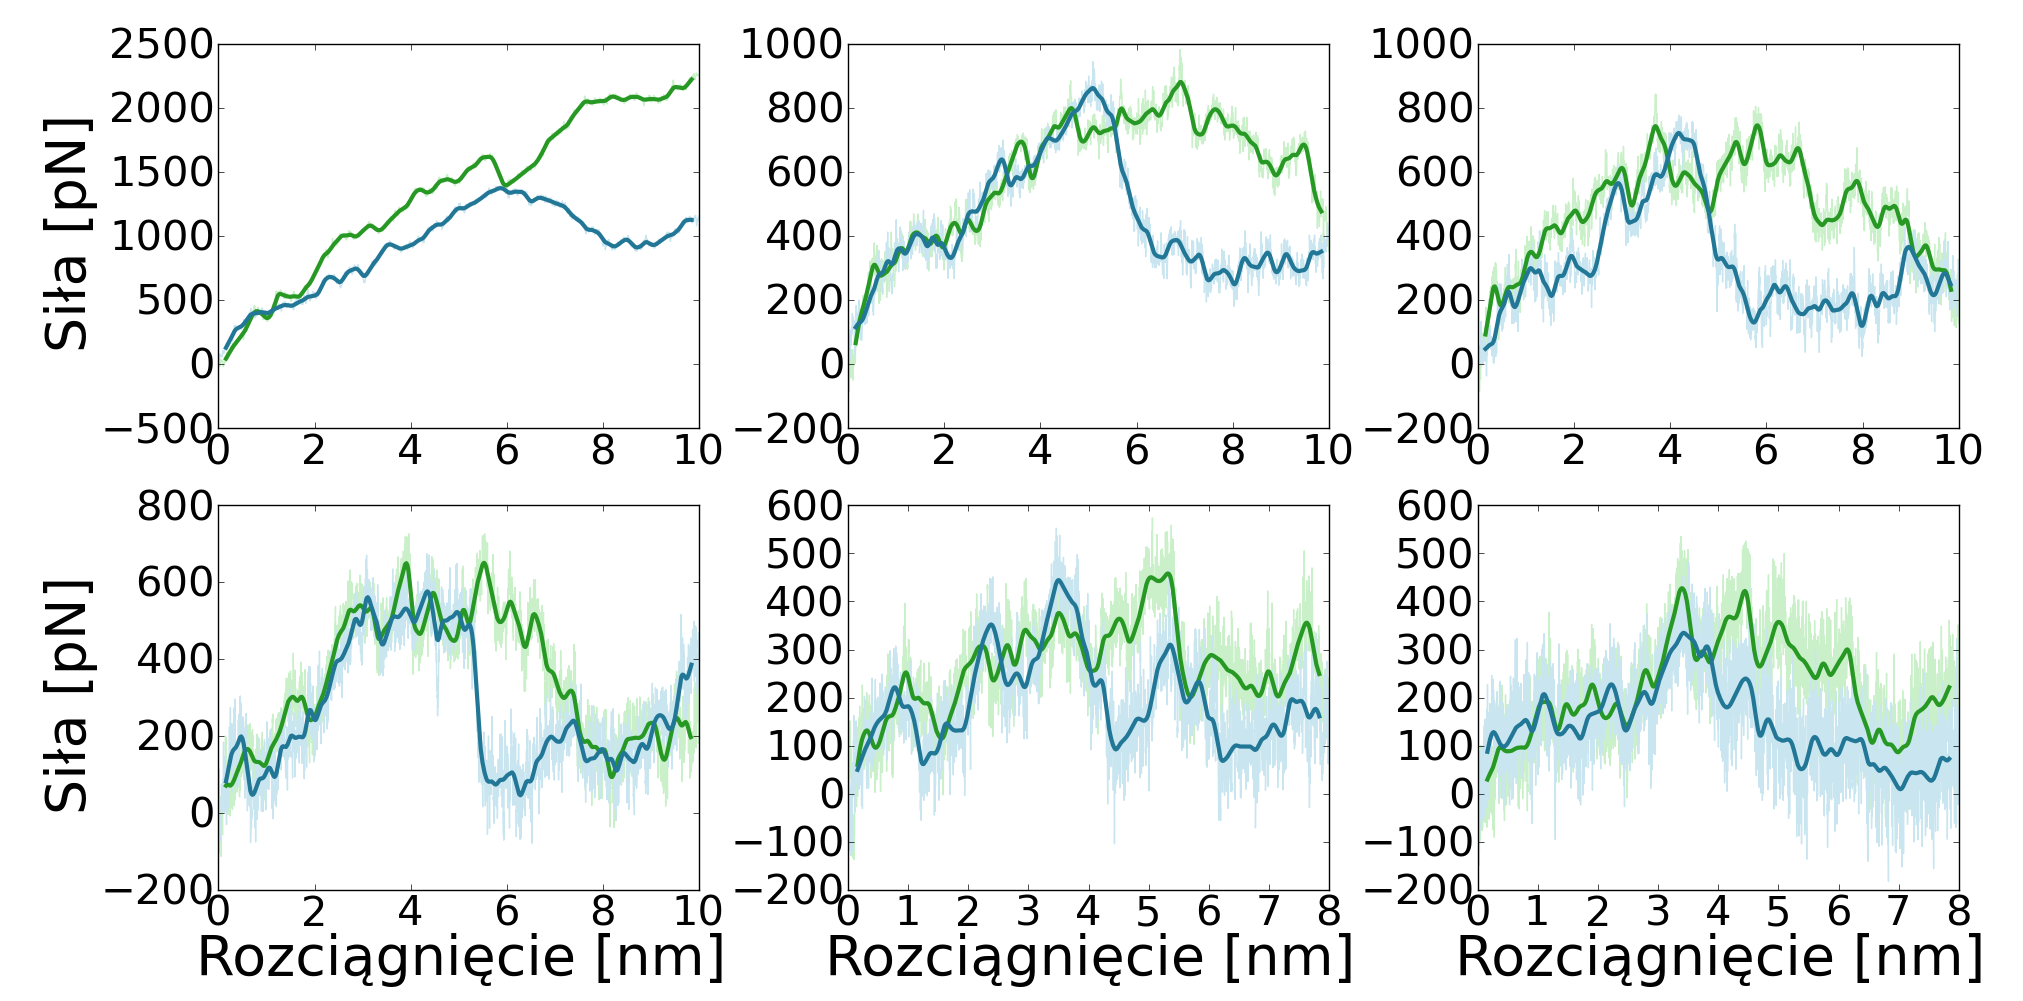
\includegraphics[width=100mm]{./rys/smooth.png}
\caption{Wygładzone krzywe zależności siły od rozciągnięcia dla 6 prędkości rozciągania.}
\end{centering}
\end{figure}

\end{center}
\end{frame}

\begin{frame}
\frametitle{Wyniki}
\begin{block}{Wyniki}
\begin{center}
\begin{table}[h]
\centering
  \begin{tabular}{| r | c | c |}
  \hline
   Prędkość  & \multicolumn{2}{|c|}{Maksymalna siła [pN]} \\
   \cline{2-3}
    [nm/ns]&  N-koniec  & C-koniec \\
  \hline
  50 & 1618 & 1372 \\
  10 & 822 & 815 \\
  5 & 745 & 720 \\
  2 & 650 & 576 \\
  0.8 & 459 & 443\\
  0.4 & 429 & 334\\
  \hline
  \end{tabular}
  \caption{Maksymalne siły rozplatania dla różnych prędkości rozciągania.}
\end{table}
\end{center}

\end{block}
\end{frame}


\begin{frame}
\frametitle{Wyniki}
\begin{center}
\begin{table}[h]
\centering
  \begin{tabular}{| c | l | l |}
  \hline
  Prędkość [nm/ns] & Czas symulacji [ns] & Czas obliczeń\\
  \hline
  50 & 0.2 & 1h15:55 \\
  10 & 1 & 4h48:31 \\
  5 & 2 & 11h57:22 \\
  2 & 5 & 21h50:17 \\
  0.8 & 10 & 2d7h56:25 \\
  0.4 & 20 & 3d15h07:03\\
  \hline
  \end{tabular}
  \caption{Czasy symulacji dla różnych prędkości rozciągania. Ramka, 0.16 nm}
\end{table}
\end{center}
\end{frame}
\section{Dopasowanie}

\begin{frame}
\frametitle{Wzory}
\begin{equation}
k_{0}=\frac{1}{\sqrt{2 \pi}}Dk_{m}^{3/2}x_{b}e^{-k_{m}x_{b}^{2}/2} 
\end{equation}
\begin{equation}
x(t)=\frac{vk_{s}}{D(k_{m}+k_{s})^{2}} (D(k_{m}+k_{s})t+e^{-D(k_{m}+k_{s}t}-1)
\end{equation}
\begin{equation}
x(\tau)=x_{b}
\end{equation}
\begin{equation}
F=-k_{s}k_{b}T(x_{b}-v \int_0^{\tau} S(t) dt)
\end{equation}
\begin{equation}
S(t)=exp(-\frac{k_{0}e^{-k_{s}x_{b}^{2}/2}}{vk_{s}x_{b}(k_{m}/(k_{m}+k_{s}))^{3/2}}(e^(k_{s}vx_{b}t-\frac{1}{2}(k_{s}vt)^{2}/(k_{m}+k_{s}))-1))
\end{equation}
\end{frame}

\begin{frame}
\frametitle{Funkcja Lamberta}
Szukając rozwiązanie równania (6) napotkano następujący problem:
\begin{equation}
c=ax + e^{-ax}
\end{equation}

Rozwiązanie tego równania znajduje się jako funkcję Lamberta (funkcja Omega):
\begin{equation}
f(w)=we^{w}
\end{equation}
Rozwiązanie równania (2) znaleziono dzięki programowi Mathematica, a rozwiązanie było liczone numerycznie.

\end{frame}

\begin{frame}
\frametitle{Kod}

\begin{block}{Procedura dopasowania}
\begin{enumerate}
\item Obliczanie $D$
\item Obliczanie $\tau$
\item Całka liczona numerycznie od 0 do $\tau$
\item Dopasowanie metodą simpleks
\end{enumerate}
\end{block}

Dopasowanie prowadzone metodą simpleks, dla funkcji sumy kwadratów różnic między wartością z symulacji, a wartością obliczoną ze wzoru.

\end{frame}


\begin{frame}
\frametitle{Dopasowanie}
\begin{center}
\begin{figure}[h]
\begin{centering}
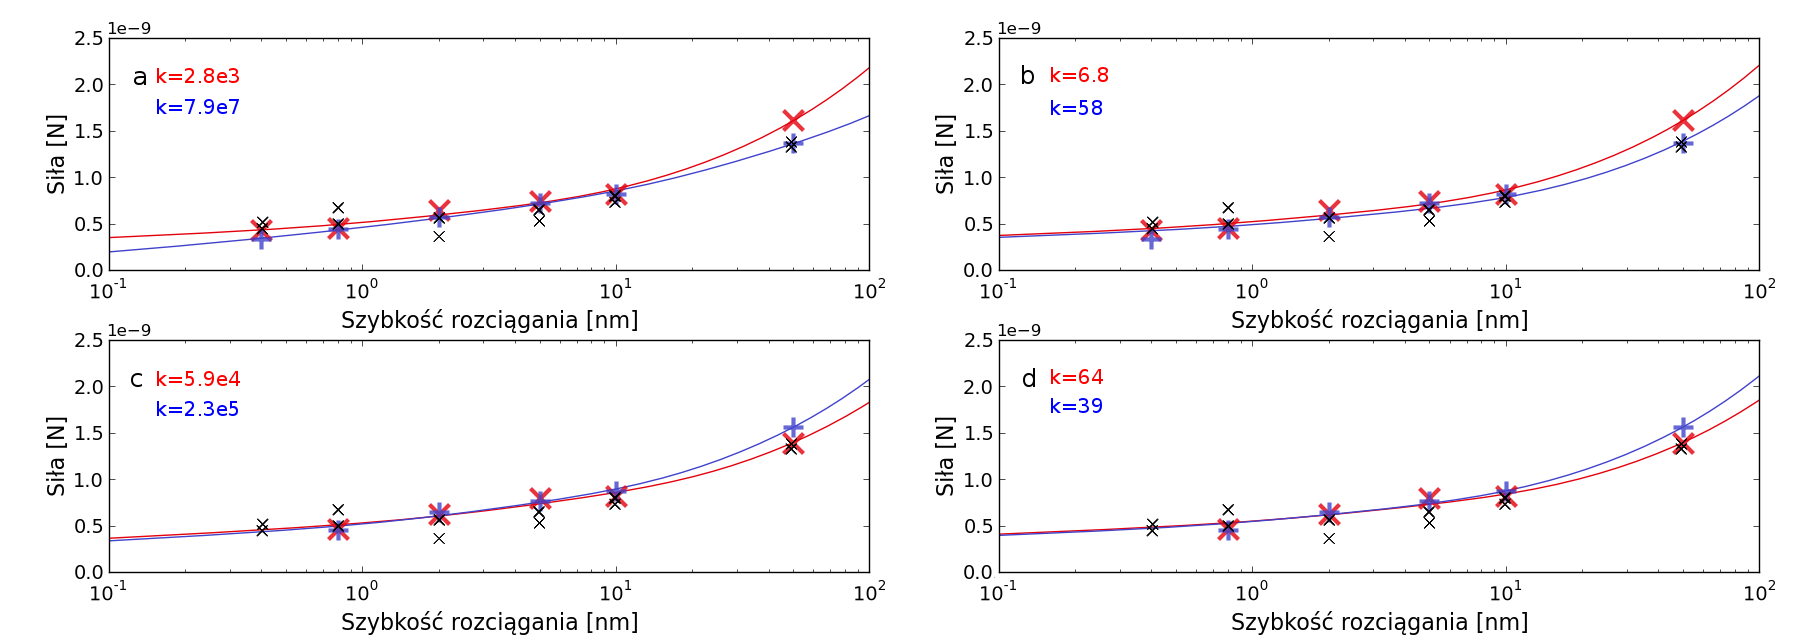
\includegraphics[width=100mm]{./poster/anal.png}
\caption{Dopasowanie do wyników z symulacji i z publikacji}
\end{centering}
\end{figure}

\end{center}
\end{frame}

\end{document}